\documentclass[cropmarks, frame, english]{idamasterthesis}

%###############################
\usepackage{luatextra}
 \usepackage{amsmath}
 \usepackage{amssymb}
 \usepackage{lmodern}
 \usepackage{uniinput-lualatex}
 \usepackage{fontspec}

% reference handling
\usepackage{cite}
\usepackage[nottoc]{tocbibind} 
\usepackage[square,comma,numbers]{natbib} 
\bibpunct{[}{]}{;}{n}{,}{,}
\usepackage{natbib}

% mathematic
\usepackage{amsmath}

% Graph
\usepackage{tikz}
\userepackage{pgf}
\usetikzlibrary{arrows,automata}
\usepackage[latin1]{inputenc}
\usepackage{verbatim}

\usepackage{flafter}
\usepackage{tikz}
\usepackage{verbatim}
\usetikzlibrary{graphdrawing}
\usetikzlibrary{graphs}
\usegdlibrary{trees}


\usepackage{caption}
\usepackage{subcaption}

%###############################

\author{Lars Niclas Jonsson}
\date{October 8, 1992}
\titleenglish{Implementation and testing of a fpt algorithm for computing the \textasciicircum + heuristic}
%\publicationmonth{June}
%\publicationyear{2015}
\supervisor{Christer B{\"a}ckstr{\H o}m}
\examiner{Christer B{\"a}ckstr{\H o}m}


\abstract{%
\S\ This is the abstract.
Yow!  Are we in the perfect mood?
Do you really think I would like not want to watch wrestling?
Half a mind is a terrible thing to waste!
Possibly your plans could have caused this.
Now Im concentrating on a specific tank battle toward
 the end of World War II!
I dont understand.
\abstractpar%
Ask me the DIFFERENCE between PHIL SILVERS and ALEXANDER HAIG!!
Earlier you said nobody is buying your urine sample bottles?
hy should I give to have this suntan to you?
}

\begin{document}

%\layout

\makeintropages

\chapter{Introduction}
This is a bachelor thesis written with the motivation to analyze an fpt algorithm for computing the *+ heuristic and compare its practical speed with "name".

Heuristic search functions are used in artificiell intelligens  to estimate the distance between a state (node) and its closest solution in automated planning and scheduling.
\section{Background and Motivation}

\subsection{Introduction}

Heuristic function are used in automated planning and scheduling to estimate the distance from a state to a goal.

An example of a planning task could be to solve the famous problem Tower of Hanoi. In the game, there is n disks and 3 rods. All disks have a different size. In the start positions, all disks are stacked in non growing order on road 1(see \ref{towers-of-hanoi} ). To solve the problem, all disks has to be stacked on road number 3 in non increasing  order. One is only allowed to lift one disk at the time and it is  not allowed to stack a bigger disk on a smaller disk.

To transform this problem to a planing task, we can create a graph where the vertexes in the graph are all the different cases that can occur in the game. There is an edge (u,v) between the vertexes u and v if it iss possible to go from state u to state v in one move. In this problem, all edges are undirected since there is always possible to go back one step. This is not the general case in planing. An example of a graph(although this is not the graph that represent the cases in Tower of Hanoi) can be seen in figure 1.2.

A path from the initial state( the start position ) to the state were all disks are at rod 3 is a solution to the problem.
If there are n disks, the shortest path has the length 2\^ n - 1 which means that the planing problem require exponential time to solve. This is the case for many planning problems and therefore, many planing problems are said to be untrackable.

\begin{figure}
\centering
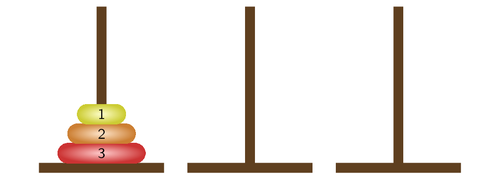
\includegraphics[width=90mm]{towers-of-hanoi.png}
\caption{Tower of Hanoi with three disks. Image source: http://www.nkonecny.com/blog/2011/11/25/towers-of-hanoi/  \label{towers-of-hanoi}}
\end{figure}


\begin{figure}
\begin{tikzpicture}[>=stealth, every node/.style={circle, draw, minimum      size=0.75cm}]
   \graph [tree layout, grow=down, fresh nodes, level distance=0.5in, sibling distance=0.5in]
    {
        A -> {
          B -> { E -> {K}, F -> {L} ,G },
          C -> { H, I -> {M  ,N} },
          D -> { J }
        }
    };

\end{tikzpicture}
\caption{A graph were the intial state is A \label{plan_graph} }
\end{figure}

\begin{figure}
\begin{tikzpicture}[>=stealth, every node/.style={circle, draw, minimum      size=0.75cm}]
   \graph [tree layout, grow=down, fresh nodes, level distance=0.5in, sibling distance=0.5in]
    {
        A -> {
          B -> { E -> {K}, F -> {L} ,G },
          C -> { H, I -> {M  ,N} },
          D -> { J }
        }
    };
\end{tikzpicture}
\caption{A graph were each vertex store a positive number which is the estimates distance from the goal. \label{heurstic_graph} }
\end{figure}





Because of that, heuristic functions are used before an actual search algorithm to estimate how far a vertex/state is from a goal. A search algorithm that are ran after a heuristic algorithm can look on the vertexes that can be reach from the current state and go to the state that was estimated to be the closest one to the goal.

In figure 3, we see the graph with numbers in each vertex which are the estimated distance for each vertex. There are two vertex that has the value 0, which means that they are both a goal to the problem. If a graph has the value  infinity, it means that the state is a dead end and no solution can be found from that state. Backtracking can be  applied if a dead end has been reached. 


In this thesis Christers algorithm [1] will calculate the delete relaxing heuristic (h+)[3] of a relaxed planing instance. 

A relaxed problem is a problem where all negative effect for all action has been remove. An example of a delete negative effect could be a robot that moves from A to B. The negative effect here is that the robot will not be at A when it is at B. If delete relaxing would been applied here, we would say that the robot is both at A and B.
 With relaxed delete instances, tower of Hanoi can be solved in linear time[1].

A relaxed planing problem is NP-complete and therefore there is not so much hope to find a fast solution to the problem,  therefor the values are usually just estimated. However, Christers algorithm is a FPT algorithm which means that the it can be calculated in polynomial speed with respect to the input size and expontial and in time seen to the number of paths in the graph that represent the planning problem.



\section{Problem definition}
Can Christer algortihm be used in practise?
\section{Limitations}

\begin{itemize}
   \item{We will only implement, execute and compare our algorithm on the planning system Fast Downward.}
   \item{Good in this case means two things: How fast the algortihm is in time and how many nodes it is visiting.}
   \item{Only binary varibels will be considered in this thesis.}
\end{itemize}

\section{Previous Work}
I am not sure what to write here! Maybe other heuristic that use relax plaining?

\chapter{Theory}
In this chapter will about the planning system Fast Downward(FD), Christers algorithm and some defintions like casual graph and tree decomponsition be explaind which is nessery for undersdanding the algorithm and how's the planner work

\section{Definitons}
\subsection{SAS Planing instance}
P = \{V, D, A, s1, sg \} is a SAS planning instance where V is the set of varibales, D(a) is the domain function for each v $\in$ V, A is a pair of a precondition pre(a) and a efftect eff(a), s1 is the initial state and s2 is the goal.
Since only binary variabels are used in this thesis, the domain for each v is \{0,1\} were v $\in$ V.

\subsection{Transition Graphs}
A transition graph G = \textless S,E \textgreater is a directed graph were S is the \textbf{state space} for the planning instance P and e = (u, v) $/in$ E if there is a action from u to v. The \textbf{state space} for V and D is S(V,D) = D(v1)*...*D(vn).
\\
If P = \{V, D, A, s1, sg \} is a planning instance and  V = \{a,b\}, A = \{(a,b), (b,c), (b,c) \}, s1 = \{a\}, sg = \{c\}, then its transition graph looks like:

\begin{tikzpicture}[->,>=stealth',shorten >=1pt,auto,node distance=2.8cm,
                    semithick]
  \tikzstyle{every state}=[fill=black,draw=none,text=white]

  \node[initial,state] (A)                    {$00$};
  \node[state]         (B) [below right of = A] {$01$};
  
  \path (A) edge              node {} (B)
            %edge              node {} (C)
        (B) edge [loop above] node {} (B)
            %edge              node {} (C)
 \end{tikzpicture}

\subsection{Causal Graphs}
-
\subsection{Tree decompostions}
A Tree decompostion of a Graph G = \lessthen V,E \biggerthen is a pair \lessthen N,T \biggerthen where N = \{ N1,N2,...,Nn\} and N\i \subset V, and

NOT COMPLETE
\section{Heuristic planing}
The planning instance P in section 2.1 were very inpcomplex and therefore also its graph (figure 1)  which makes it easy to solve. In reality, a planning instance can have 10000 varibales and actions which is not solvable today since planning is a NP-problem

\section{Fast Wordward}
Fast Wordward(FD) is a planning system that read PDDL-code as its input and calculate a solution to the planning problem the PDDL code descripe. 
When FD solves a problem, it goes thorugh 3 different phases(translation, knowledge compilation and search. 

The first phase takes the PDDL-code as its input and return a multi-valued planning task. 
 This phase takes the outpout from phase 1 as its input and generates four data structures: Domain transition graphs, Causal graph, the successor generator, and the axiom evualtor. 
In the last phase is the actual searching done. There are 3 search algortihm in FD, two of this are use a heuistic algorithm but the last one does not. 



\cite{Backstrom2004a}
\cite{Bodlaender1993}
\cite{Helmert2006}
\cite{Hoffmann2001}

%#####
\bibliographystyle{plain}
\bibliography{ref}

\end{document}
